\section{Introduzione}\todo{prima bozza.. ancora da rileggere completamente}

Il seguente progetto ha come obiettivo quello di realizzare un'applicazione che consenta di ricavare automaticamente la rappresentazione in \LaTeX \;di un circuito elettrico realizzato con il software di simulazione LTSpice (\href{https://www.analog.com/en/design-center/design-tools-and-calculators/ltspice-simulator.html}{Analog Devices}). In particolare, il pacchetto \href{https://it.overleaf.com/learn/latex/CircuiTikz_package}{CircuiTikz} permette di rappresentare in Latex un circuito elettrico. Inoltre, LTSpice produce un file con estensione .asc che contiene tutte le informazioni utili alla rappresentazione grafica dei componenti, come ad esempio la posizione assoluta dei vari elementi circuitali, la loro etichetta e il loro valore. L'idea alla base di questo progetto è quella di utilizzare le informazioni contenute nel file .asc e il pacchetto CircuiTikz per ottenere una rappresentazione in Latex del circuito. Una volta ottenuto il file .tex, si utilizza lo strumento \texttt{pdflatex} (distribuito con il compilatore MikTex) per generare un documento pdf.
\subsection{Tecnologie utilizzate}
Per lo sviluppo di questo progetto si sono utilizzate le seguenti tecnologie:
\begin{itemize}
	\item \texttt{ANTLRWorks 1.5.2}, per la generazione del lexer e del parser nel linguaggio java;
	\item libreria java \texttt{antlr-complete} versione 3.4;
	\item libreria \texttt{CircuiTikz} e il compilatore \texttt{MikTex}, per la generazione del codice Latex e del documento pdf;
	\item \texttt{Eclipse IDE}, per la creazione del progetto java del lexer e del parser e la compilazione;
	\item framework Qt, per la creazione dell'app client;
	\item \texttt{GitHub}, per il versioning del codice;
\end{itemize}
\subsection{LTSpice}
LTSpice è un software molto utilizzato in ambito accademico e lavorativo per effettuare simulazione di circuiti elettrici. L'interazione con il programma avviene tramite un'interfaccia grafica che permette di inserire i componenti, assegnare loro un valore e un identificativo e definire i parametri di simulazione (\Fig\ref{fig:ltspice}).
\begin{figure}[h!]
	\centering
	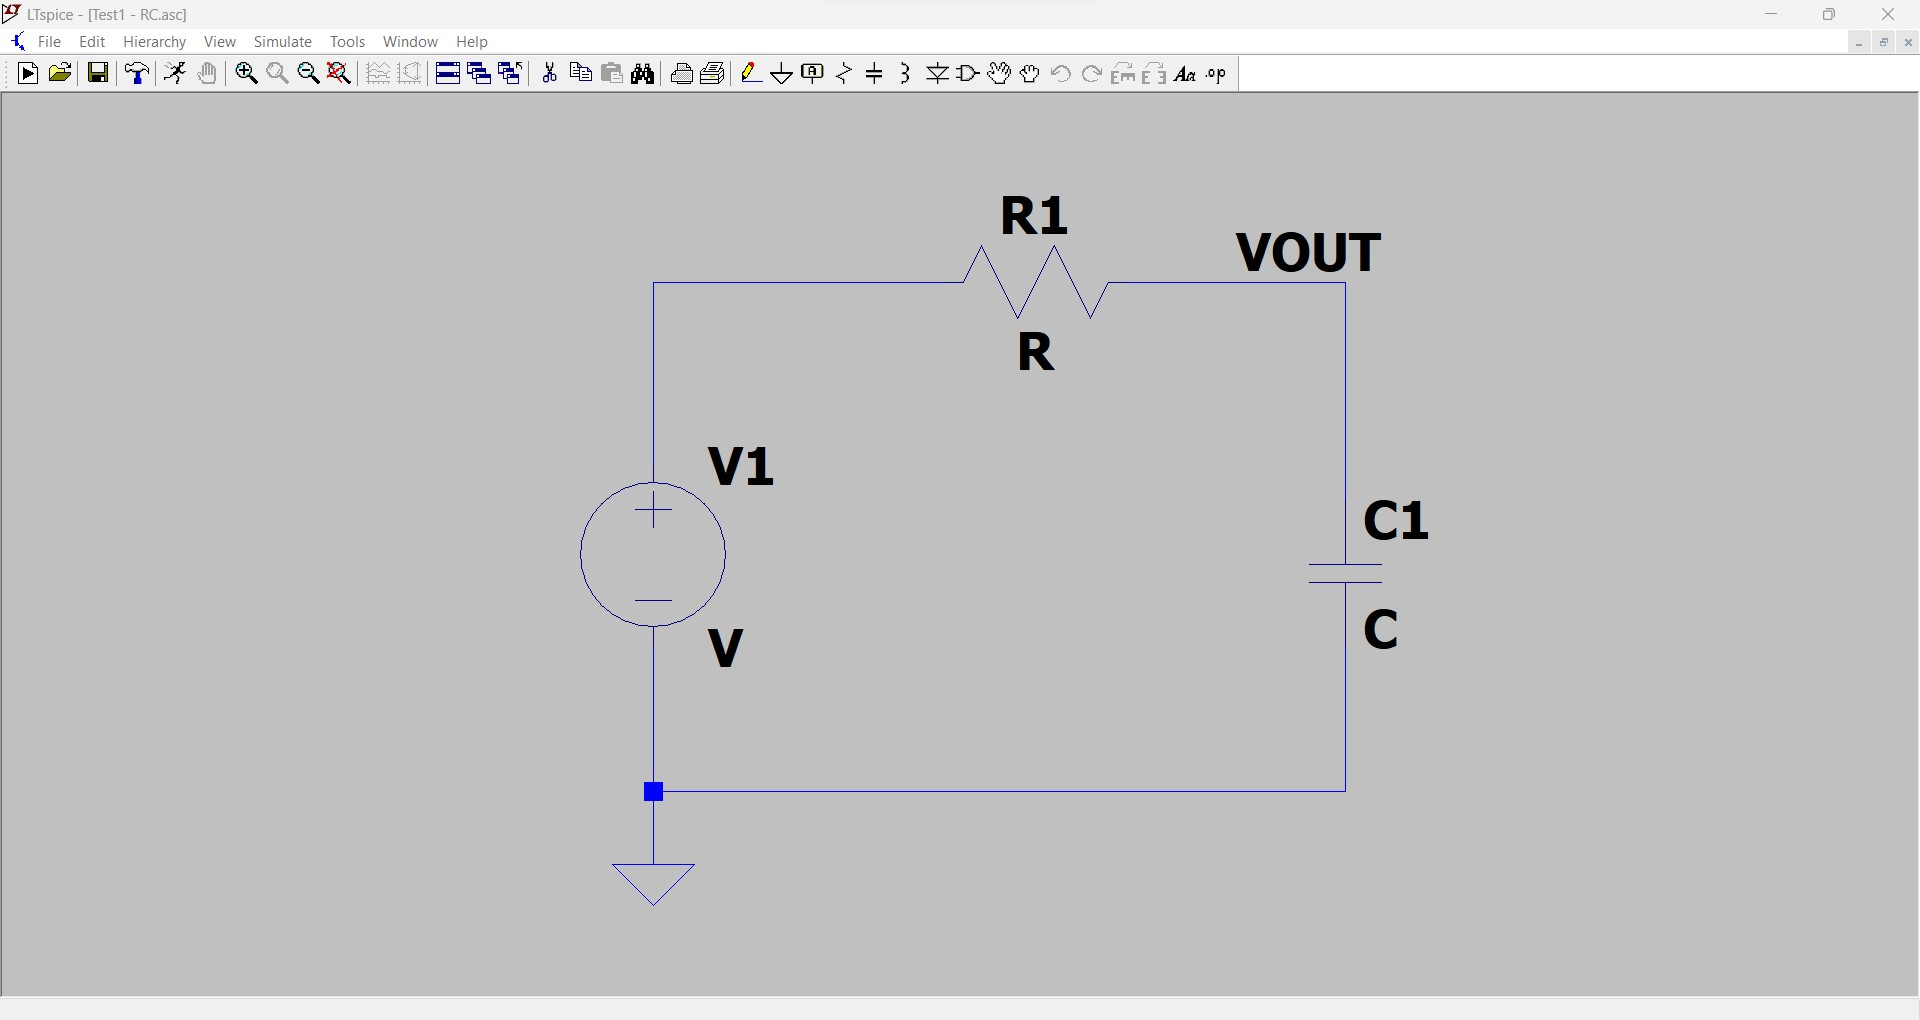
\includegraphics[width=\textwidth]{./ImageFiles/LTSpice.jpg}
	\caption{Schermata principale di LTSpice.}
	\label{fig:ltspice}
\end{figure}
Il motore di simulazione è basato sul programma SPICE (\textit{Simulation Program with Integrated Circuit Emphasis}) che riceve in input una \texttt{netlist}, ossia una rappresentazione testuale del circuito, e produce in output i risultati di simulazione. LTSpice crea automaticamente la \texttt{netlist} a partire dalla rappresentazione grafica del circuito. Per esempio, il circuito in figura \ref{fig:ltspice} genera la seguente netlist:
\lstinputlisting[language=Octave]{./OtherFiles/netlist.txt}
Inoltre, il programma salva il circuito in un file con estensione .asc che contiene tutte le informazioni per rappresentare in modo grafico il circuito. Di seguito si riporta il file .asc prodotto dal circuito in figura \ref{fig:ltspice}.
\lstinputlisting[language=Octave]{./OtherFiles/asc.txt}
Come si può notare, in questo file non vengono riportate informazioni sulla simulazione da eseguire ma bensì la posizione dei collegamenti e dei componenti, la posizione di label associate ed eventuali attributi. In particolare, le principali parole chiave che si possono riconoscere sono: \todo{descrizione generica. c'è dopo la grammatica}
\begin{itemize}
	\item VERSION, rappresenta la versione del sistema utilizzato\todo{non è la versione di ltspice}; per il progetto verrà considerata solamente la versione 4;
	\item SHEET, definisce il numero del figlio di lavoro utilizzato e le relative dimensioni;
	\item WIRE, indica un filo di collegamento; seguono le coordinate x,y assolute dei relativi capi;
	\item SYMBOL, rappresenta un componente; viene indicato di seguito la tipologia, la posizione assoluta in coordinate x,y e l'eventuale rotazione o mirror; è possibile indicare una rotazione di 0°, 90°, 180°, 270° o un'operazione di mirror di 0°, 90°, 180° e 270°;
	\item SYMATTR, permette di indicare eventuali attributi riferiti a un simbolo come il nome, il valore, i parametri di eventuali componenti parassiti o indicare il produttore del componente;
	\item WINDOW, indica la posizione della label associata a un componente (il nome o il valore) nel caso di rotazioni e mirror;
	\item FLAG, definisce la posizione e il contenuto di eventuali label associati a dei collegamenti in un circuito; viene utilizzata anche per indicare la massa (indicando come nome della label 0);
	\item IOPIN, indicano label di ingresso o uscita nel circuito. 
\end{itemize}
Tutte le coordinate sono espresse attraverso numeri interi e le parole chiave sono interpretate in modo \textit{case insensitive}. Il formato di codifica del file è \texttt{ISO-8859-1} e accetta qualsiasi carattere \texttt{UNICODE} all'interno delle label e dei nomi dei componenti. Le parole chiave e i relativi parametri sono separati da degli spazi bianchi. LTSpice è insensibile al numero di spazi tra i diversi token e di eventuali \textit{newline}. Tuttavia, il file .asc in output a LTSpice è formattato mantenendo un unico spazio tra ogni token e andando a capo ad ogni parola chiave.

\section{ltspice2circuitikz}
\todo{spiegazione generale della struttura della applicazione}
\begin{figure}[h!]
	\centering
	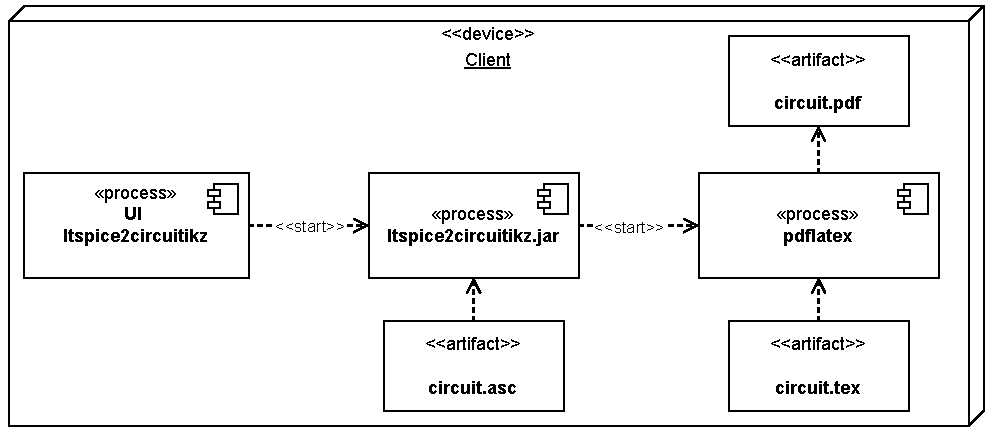
\includegraphics[width=0.5\textwidth]{./ImageFiles/deploy diagram.pdf}
	\caption{Deploy diagram del sistema.}
	\label{fig:deploy_diagram}
\end{figure}

\begin{figure}[h!]
	\centering
	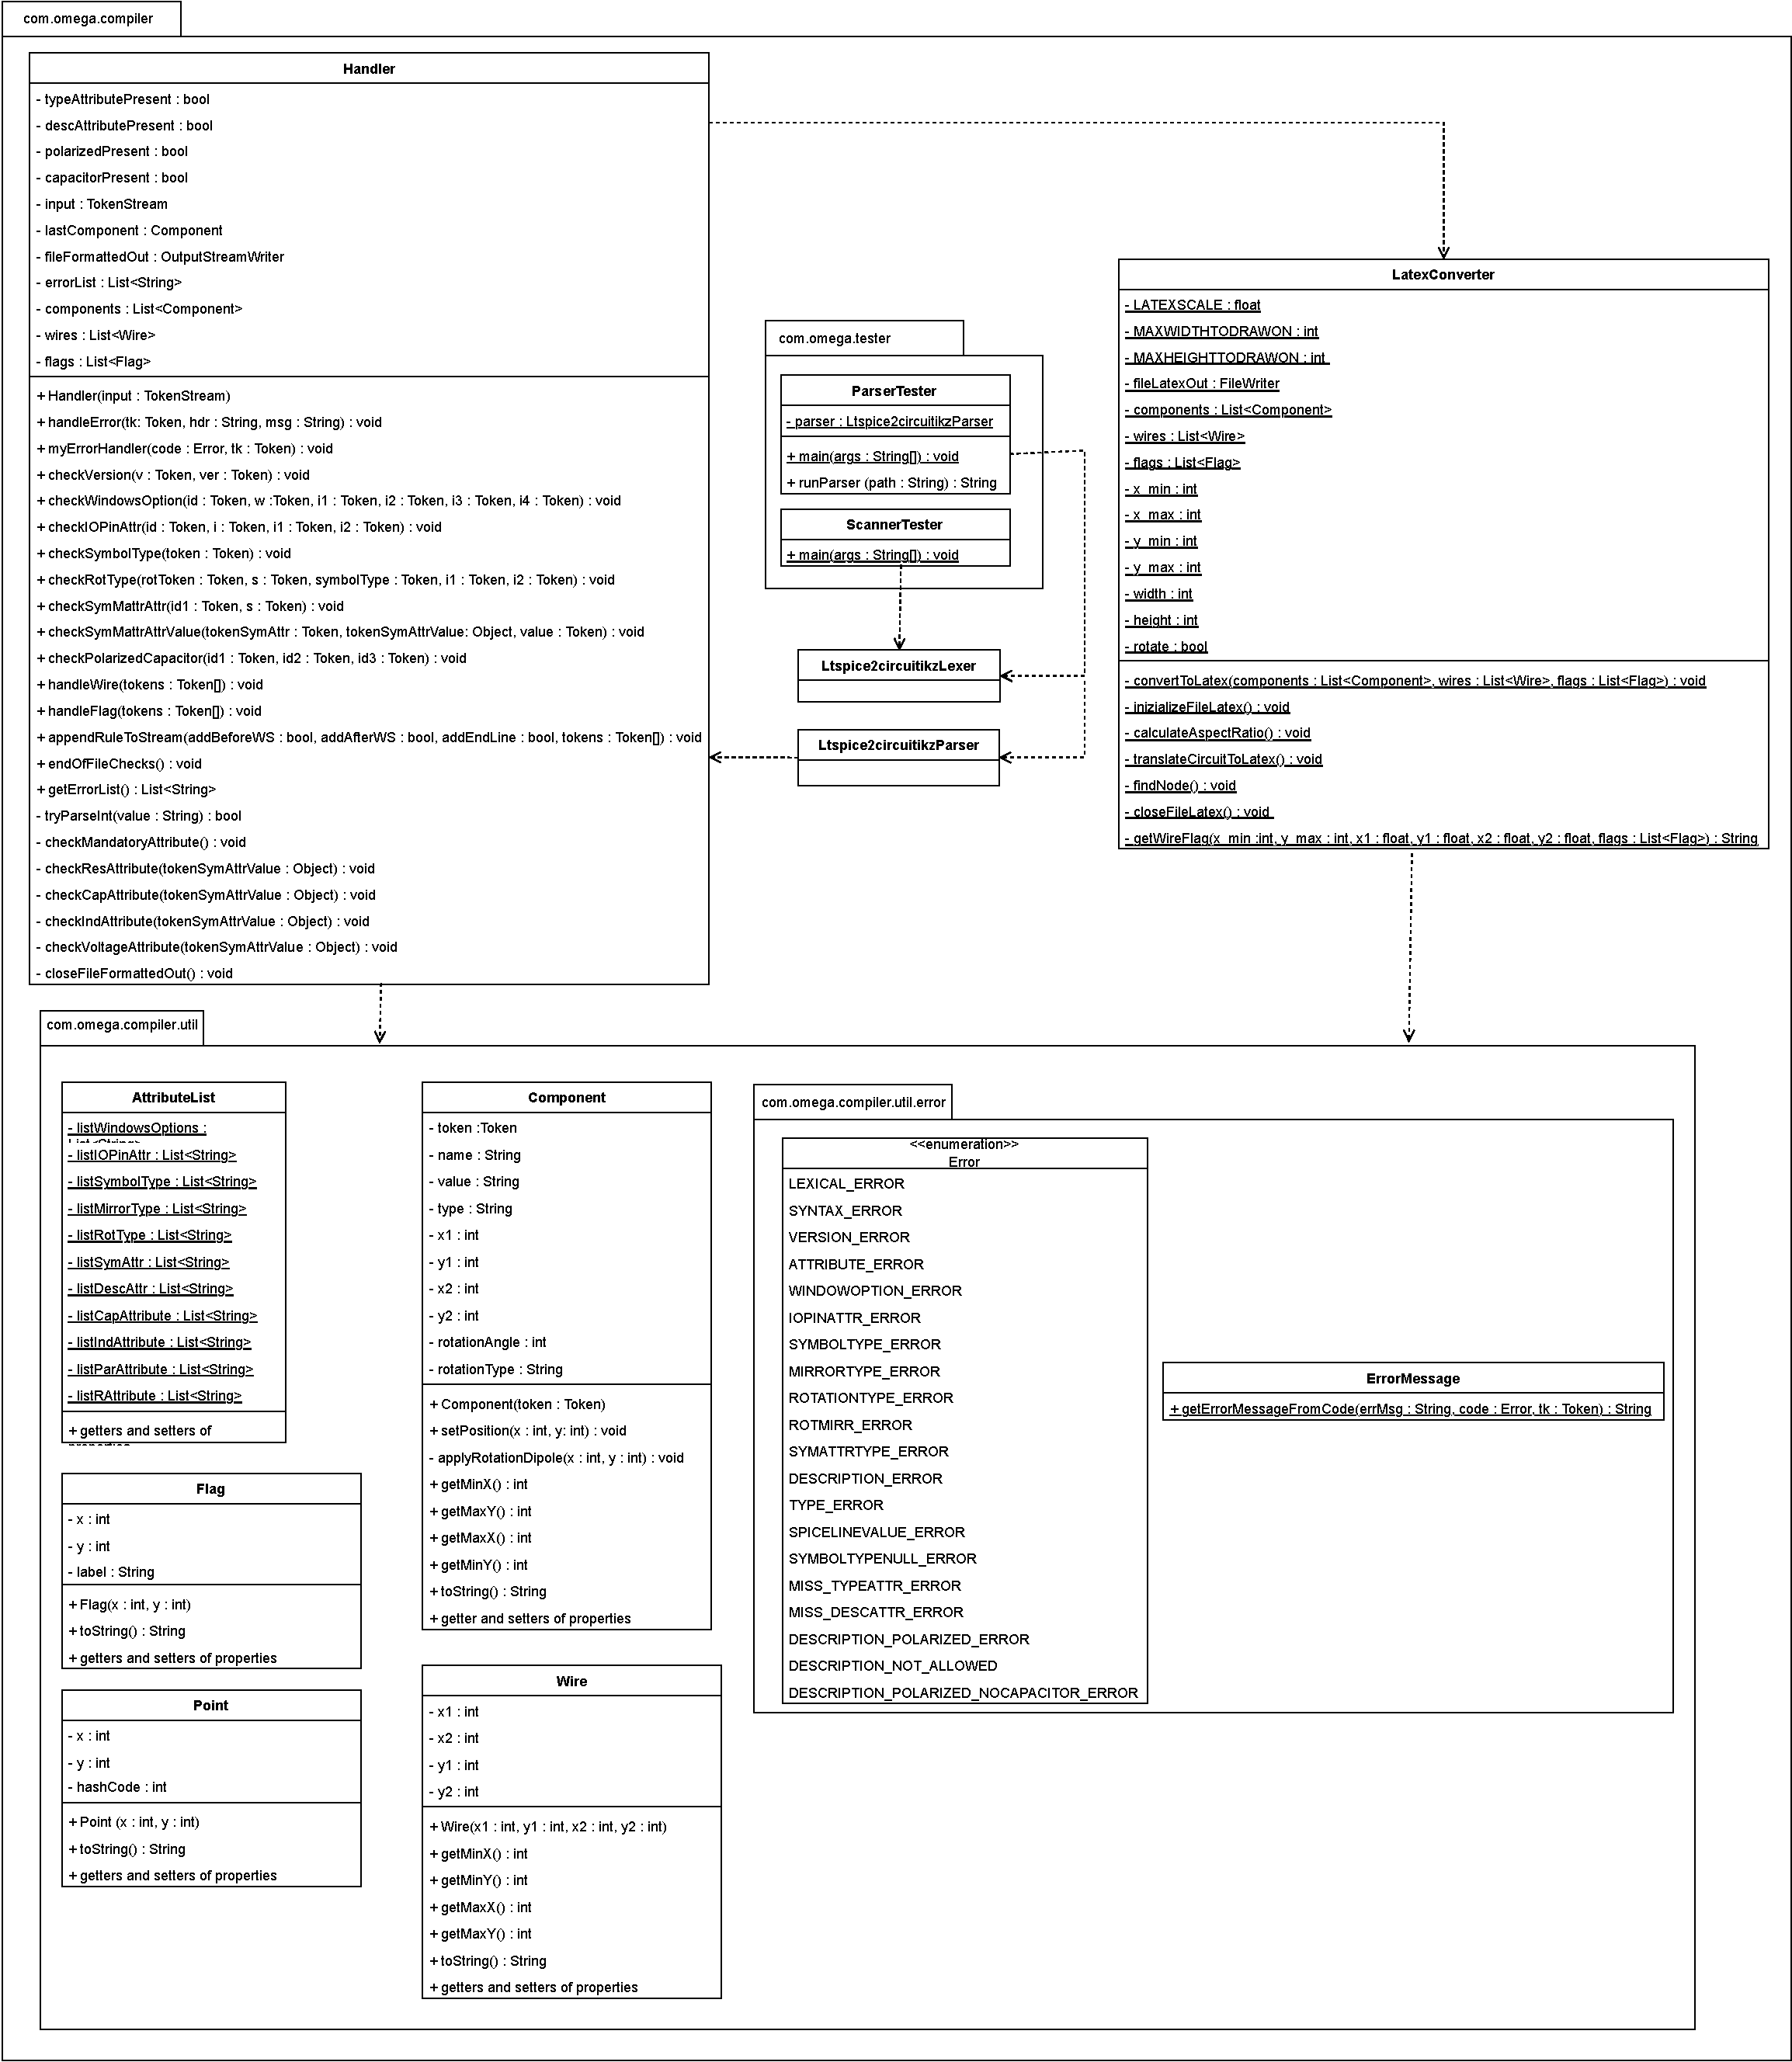
\includegraphics[width=\textwidth]{./ImageFiles/class and package diagram.pdf}
	\caption{Class and Package Diagram dell'applicazione.}
	\label{fig:class_diagram}
\end{figure}


\subsubsection{Lexer e Parser}
L'applicazione realizzata si basa su un lexer e un parser LL(1) generato nel linguaggio Java grazie al tool AntlrWorks, che permette di leggere ed interpretare un file .asc e di effettuare la traduzione in un file .tex tramite delle azioni semantiche. Per definire la grammatica utile al parsing del file .asc è stato eseguito un processo di reverse engeneering, analizzando il file generato da LTSpice con dei circuiti di esempio. Di seguito si riportano i token identificati e le regole sintattiche ricavate dall'analisi dei file .asc.
\lstinputlisting[]{./OtherFiles/grammatica non decorata.txt}
In particolare, si è notato che il programma non generava errore all'apertura del file se:
\begin{itemize}
	\item le parole chiave erano scritte in caratteri minuscoli o in una qualsiasi combinazione di caratteri minuscoli e maiuscoli;
	\item venivano aggiunti degli spazi bianchi o dei caratteri di terminazione di riga tra le parole;\todo{come si dice il carcatte slash/n a parole?!?!?}
\end{itemize}
Per mantenere coerente la grammatica con queste regole, sono stati considerati come separatori tra i diversi token i caratteri di spazio bianco e di terminazione di riga. Inoltre, le parole chiave sono state rese invarianti rispetto al carattere delle lettere (lower o upper case). La grammatica completa si compone di nove parole chiavi: VERSION, SHEET, WIRE, SYMBOL, SYMATTR, simbolo di assegnamento (=), WINDOW e IOPIN. Ulteriori controlli sulle possibili strutture sono state inserite nella semantica discussa successivamente. Inoltre, LTSpice accetta l'inserimento di qualunque carattere \texttt{UNICODE} nelle label dei componenti. Per questo motivo sono stati aggiunti i token per la lettura dei caratteri speciali, dell'alfabeto greco e dell'alfabeto cirillico.

\subsection{Semantica}
Per gestire le azioni semantiche è stata predisposta la classe \texttt{Handler.java} che racchiude la definizione dei metodi utilizzati per i controlli semantici e le operazioni di traduzione. Di seguito si riporta la grammatica decorata con le operazioni semantiche.
\lstinputlisting[]{./OtherFiles/grammatica decorata.txt}

\noindent
Inizialmente, nel costruttore della classe vengono inizializzate alcune strutture dati che verranno utilizzate per gestire la traduzione. In particolare, vengono create le liste \texttt{components}, \texttt{wires} e \texttt{flags} che servono a memorizzare i componenti letti in modo incrementale durante l'analisi del file in input; viene inizializzata anche una lista che conterrà gli errori lessicali, sintattici e semantici. Inoltre, viene creata una cartella con il nome \texttt{circuit\_output} e un file denominato \texttt{formatted\_circuit.asc} che conterrà la descrizione del circuito in formato LTSpice formattato correttamente. Infatti, come già descritto in precedenza, l'inserimento di spazi bianchi e caratteri di terminazione di linea non precludono la possibilità di interpretare correttamente il file. Per questo motivo, ogni qualvolta viene letto un token o un'insieme di token essi sono accodati al file \texttt{formatted\_circuit.asc} grazie alla funzione \texttt{appendRuleToStream} dichiarata nell'handler. Questa funzione ha come argomenti l'insieme dei token da scrivere sul file e alcuni parametri booleani per descrivere come devono essere formattati nel file (aggiungere uno spazio prima o dopo ogni token e al termine il carattere di \textbackslash n al termine della riga). 

\noindent
Un altro campo importante nella classe \texttt{Handler.h} è lastComponent. Esso è di tipo Component, una classe contenuta nel package \texttt{com.omega.compiler.util} che contiene tutte le informazioni relative a un componente. Questa variabile è utilizzata per mantenere memoria dell'ultimo componente letto: in questo modo, è possibile poi effettuare dei controlli sulle regole che vengono lette successivamente e che si riferiscono a quel componete. Essa viene inizializzata nel metodo \texttt{checkSymbolType} chiamato quando si incontra la parola chiave \texttt{SYMBOL} nella regola sintattica \texttt{symbolRule}.
\todo{che altri metodi descrivere...  mi concentrerei più sui metodi di traduzione }

\noindent
Al termine della lettura di tutto il contenuto del file .asc in input, se non ci sono stati errori viene chiamato il metodo statico \texttt{convertToLatex} della classe \texttt{LatexConverter} che inizia il processo di traduzione. Inoltre, si procede alla chiusura del file \texttt{formatted\_circuit.asc}.

\subsection{Traduzione}
La classe \texttt{LatexConverter} contiene i metodi necessari alla traduzione del circuito per la rappresentazione Latex. Il metodo \texttt{convertToLatex} chiamato dall'handler, riceve in ingresso la lista dei componenti, dei collegamenti e delle etichette ricavate dal file in ingresso. Successivamente, viene chiamato il metodo \texttt{calculateAspectRatio} che consente di calcolare i valori massimi e minimi delle coordinate x e y di tutti gli elementi del circuito e viene calcolata l'altezza e la larghezza del circuito nel sistema di riferimento di LTSpice. Se l'altezza è minore della larghezza allora il circuito verrà rappresentato su un foglio in modalità \textit{landscape}. Nella figura \ref{fig:sdr} sono mostrati i sistema di riferimenti utilizzati in LTSpice e in Latex. Non è conosciuta la posizione assoluta del sistema di riferimento in LTSpice rispetto alla finestra visualizzata.
\begin{figure}[h!]
	\centering
	a)
	\begin{minipage}{.460\textwidth}
		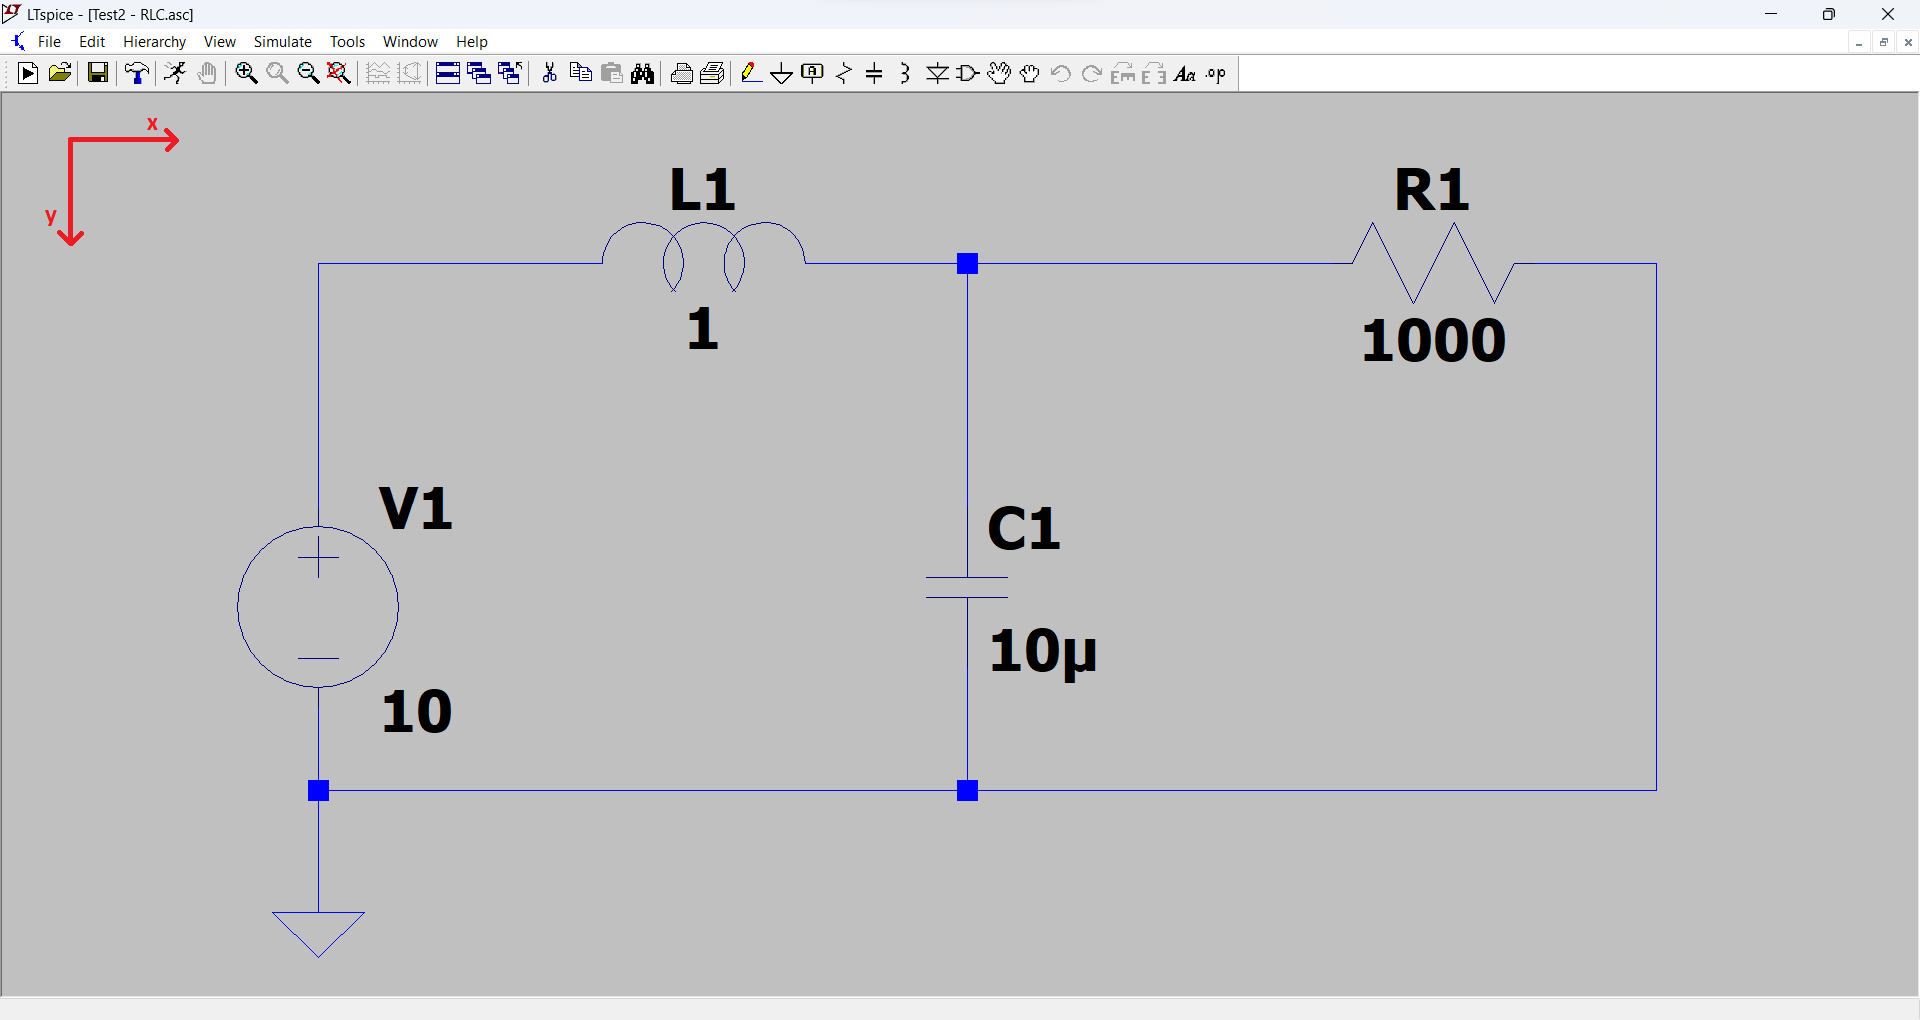
\includegraphics[width=\linewidth]{./ImageFiles/sdr-lt.png}
	\end{minipage}
	b)
	\begin{minipage}{.460\textwidth}
		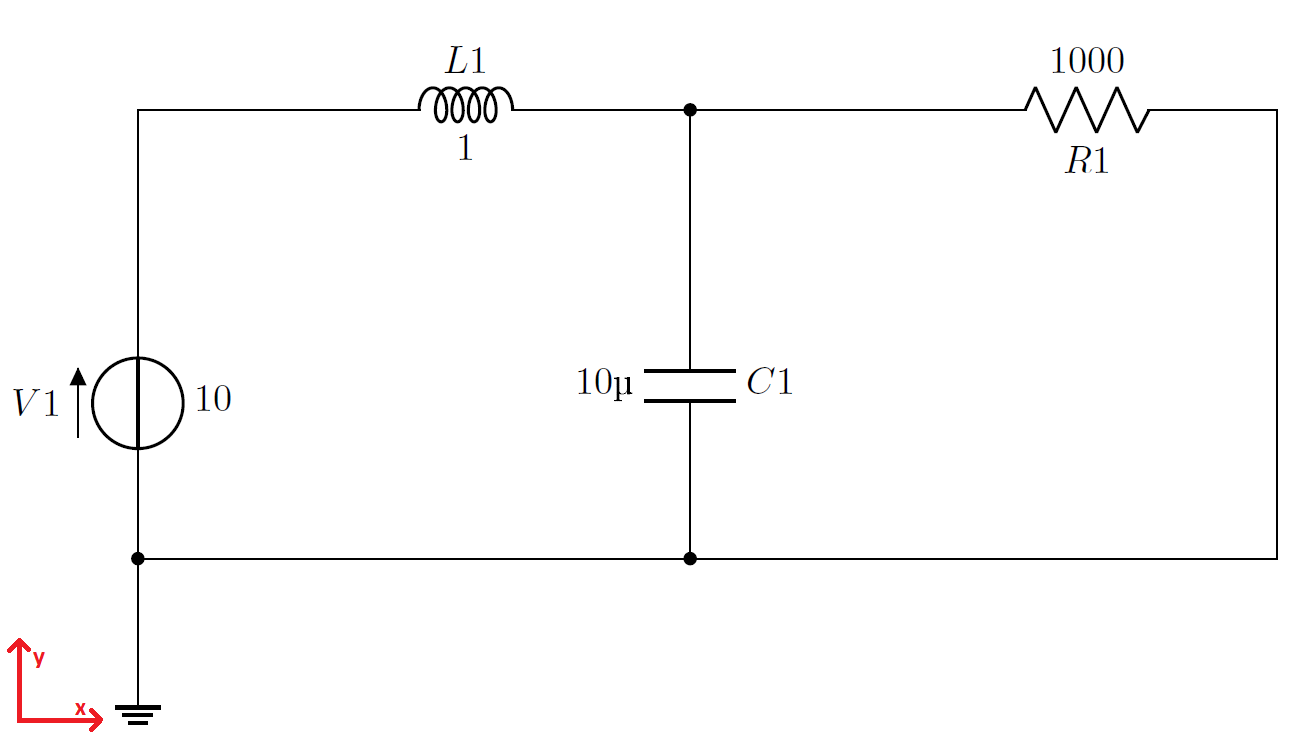
\includegraphics[width=\linewidth]{./ImageFiles/sdr-latex.png}
	\end{minipage}
	\caption{Sistemi di riferimento delle coordinate x e y in LTSpice e in Latex.}
	\label{fig:sdr}
\end{figure}

\noindent
Viene quindi creata la cartella \texttt{latex\_output} e il file \texttt{translated\_circuit.tex} che conterrà la traduzione in Latex del circuito. Dapprima, viene scritto il preambolo che contiene la descrizione del tipo di documento, la dimensione del foglio e l'import del pacchetto \texttt{circuitikz}. Queste informazioni verranno utilizzate dal compilatore \texttt{MikTex} durante la generazione del file pdf.

\noindent
Il passo successivo consiste nella vera e propria traduzione del circuito in Latex effettuata dalla funzione \texttt{translateCircuitToLatex}. Viene calcolato il fattore di scala (memorizzato nella variabile \texttt{LATEXSCALE}) tra le coordinate espresse nel sistema di riferimento di LTSpice e quello di Latex; \todo{se riesci a dire come che non ricordo :)}. Successivamente, vengono tradotti tutti i componenti, i collegamenti e i label inseriti nelle liste \texttt{components}, \texttt{wires} e \texttt{flags}; questa operazione richiede di recuperare le coordinate x e y degli estremi di collegamento di ogni componente e effettuare una rototraslazione per riportare le coordinate nel sistema di riferimento di Latex. In particolare, alla coordinata x viene sottratta la x minima calcolata nella funzione \texttt{calculateAspectRatio} mentre alla y viene sottratta la coordinata y massima, anch'essa calcolata precedentemente. Le coordinate y vengono poi invertite. Infine, tutte le coordinate vengono scalate con il fattore di scala \texttt{LATEXSCALE} calcolato precedentemente. Il comando Latex utilizzato per disegnare un componente secondo la libreria \texttt{circuitikz} è \texttt{draw} con la seguente struttura:
\begin{itemize}
	\item \textbackslash draw (x1,y1) to[$\langle$type$\rangle$=$\langle$name$\rangle$, a=$\langle$value$\rangle$] (x2,y2), per disegnare un componente; il $\langle$type$\rangle$ può essere R, C, eC, L, Do o vsource per indicare una resistenza, un capacitore, un capacitore polarizzato, una induttanza, un diodo e un generatore di tensione; $\langle$name$\rangle$ e $\langle$value$\rangle$ corrispondono al nome e al valore del componente;
	\item \textbackslash draw (x1,y1) to[short, l=$\langle$label$\rangle$] (x2,y2), traccia un filo di collegamento dal punto (x1,y1) al punto (x2,y2) e associa eventualmente una label $\langle$label$\rangle$ al collegamento; questa label viene ricercata nella lista \texttt{flags}, cercando una flag che abbia le stesse coordinate di uno dei capi del collegamento;
	\item \textbackslash draw (x,y) to (x,y) node[ground]{}, inserisce un nodo di massa nel punto (x,y); i nodi di massa in LTSpice sono rappresentati da dei flag con valore 0;
	\item \textbackslash draw (x,y) to[short, -*] (x,y), permette di rimarcare un nodo come punto di collegamento tra tre fili; vengono ricavati cercando l'intersezione di almeno tre collegamenti grazie alla funzione \texttt{findNode};
\end{itemize}
Dopo aver terminato la traduzione, la funzione \texttt{closeFileLatex} esegue le operazioni di chiusura del file latex, dopo aver inserito l'epilogo. Successivamente, crea attiva un nuovo processo \texttt{pdflatex} al quale passa il nome del file da cui generare il pdf (\texttt{translated\_circuit.tex}). Se l'operazione va a buon fine, viene prodotto nella cartella \texttt{latex\_output} il pdf con la rappresentazione del circuito.

\todo{gestione errori}

\section{Client app}
\todo{inserirei due parole tecniche sulla applicazione client}

\section{Esempi e sviluppi futuri}